\chapter{Biologi Konservasi}\label{ch:b3:conservation-biology}

Pada 1813 Audubon menyaksikan sekawanan merpati penumpang melintasi
Kentucky selama tiga hari, menggelapkan langitnya; barangkali ada lima
miliar ekor, seperempat dari seluruh burung Amerika Utara. Pada
1~September 1914 yang terakhir, seekor betina bernama Martha, mati di
Kebun Binatang Cincinnati. Spesiesnya tidak langka ketika kemerosotannya
bermula; ia dipanen dengan muatan kereta api, dan hutannya ditebang, lalu
seekor burung yang hanya berbiak di dalam koloni raksasa tidak dapat lagi
berbiak begitu koloninya menipis di bawah suatu ukuran yang tidak seorang
pun mengukurnya. Pada 1995 kakapo, seekor burung nuri malam yang tidak
dapat terbang dari Selandia Baru, tinggal lima puluh satu ekor; tiap ekor
sejak itu telah dinamai, ditimbang, dipasangi pemancar dan, pada saat
yang tepat, disuguhi makanan tambahan, dan kini ada dua ratus lima puluh.
Pada tahun yang sama tiga puluh satu serigala kelabu dilepaskan ke
Yellowstone, tujuh puluh tahun setelah kawanan asli terakhirnya ditembak;
dalam dua dasawarsa rusa wapitinya telah berpindah, dedalunya kembali
tumbuh di sepanjang sungainya, dan berang-berangnya bersama mereka.
Biologi konservasi adalah penerapan genetika populasi, ekologi dan
perilaku dari buku ini pada satu pertanyaan praktis --- bagaimana menjaga
spesies agar tidak lenyap --- dan aritmetikanya adalah aritmetika bilangan
kecil.

\section{Mengapa populasi kecil mati}

\begin{definition}[Risiko kekecilan]\label{def:b3:conservation-biology:small}
\index{stokastisitas demografi}\index{stokastisitas lingkungan}%
\index{efek Allee}\index{pusaran kepunahan}\index{populasi layak minimum}
Sebuah populasi besar merosot bila laju kematiannya melampaui
laju kelahirannya; populasi kecil dapat lenyap tanpa perubahan pada keduanya.
\emph{Stokastisitas demografi} adalah peluang bahwa, di antara beberapa
individu, yang mati kebetulan lebih banyak daripada yang lahir, atau semua
yang selamat berkelamin jantan: ia berarti di bawah beberapa lusin ekor.
\emph{Stokastisitas lingkungan} --- musim dingin yang buruk, kekeringan,
suatu penyakit --- menerpa tiap individu sekaligus, dan populasi beberapa
ratus yang akan dilewati populasi besar dapat tersapu habis;
\emph{malapetaka} adalah ekornya. \emph{Efek Allee} membuat laju
pertumbuhan per kapita jatuh pada kerapatan rendah --- pasangan tidak
dapat ditemukan, pembiak berkoloni tidak dapat bersarang, kawanan tidak
dapat membela anaknya, kawanan merpati penumpang tidak dapat menjenuhkan
pemangsa yang mengambil anakannya --- sehingga di bawah kerapatan ambang
populasinya merosot menuju nol dengan sendirinya. Dan di bawah beberapa
ratus, proses genetik pada bagian berikutnya menurunkan kebugarannya dari
generasi ke generasi. Semuanya saling memberi makan: populasi yang lebih
kecil kehilangan keragaman, menjadi kurang subur, tumbuh mengecil, lebih
mungkin tertimpa kebetulan, lalu kehilangan lebih banyak lagi --- yaitu
\emph{pusaran kepunahan} (Gilpin dan Soulé, 1986). \emph{Populasi layak
minimum} adalah ukuran yang di atasnya peluang kepunahan sepanjang
cakrawala yang dinyatakan (katakanlah \qty{5}{\%} dalam satu abad) dapat
diterima; ia bergantung pada biologi spesiesnya dan pada seberapa
berubah-ubah lingkungannya, dan biasanya berada dalam ribuan.
\end{definition}

\begin{omfigure}
\begin{tikzpicture}[every node/.style={font=\scriptsize}, >=stealth]
  \node[draw, thick, rounded corners, fill=omThm!20, align=center] (small) at (0,0) {populasi\\menjadi kecil};
  \node[draw, thick, rounded corners, fill=omDef!20, align=center] (drift) at (3.4,1.6) {hanyutan dan silang dalam:\\keragaman hilang, $F$ naik};
  \node[draw, thick, rounded corners, fill=omDef!20, align=center] (fit) at (6.8,0) {kebugaran turun:\\anak lebih sedikit, penyakit lebih banyak};
  \node[draw, thick, rounded corners, fill=omDef!20, align=center] (chance) at (3.4,-1.6) {kebetulan demografis dan lingkungan\\menggigit lebih keras};
  \node[draw, thick, rounded corners, fill=omProp!25, align=center] (allee) at (9.9,0) {efek Allee:\\pertumbuhan negatif};
  \draw[->, very thick] (small) -- (drift); \draw[->, very thick] (drift) -- (fit); \draw[->, very thick] (fit) -- (chance); \draw[->, very thick] (chance) -- (small);
  \draw[->, thick, omProp!80!black] (fit) -- (allee); \draw[->, thick, omProp!80!black] (allee.south) .. controls (9.9,-3) and (0,-3.4) .. (small.south);
  \node[align=center, font=\tiny] at (3.4,0) {pusaran kepunahan:\\tiap putaran menyusutkan\\populasinya lalu mempercepat putaran berikutnya};
  \node[left, align=right, font=\tiny] at (-1.7,1.5) {hilangnya habitat,\\panen, pemangsa asing,\\penyakit mendorong\\populasinya masuk};
  \draw[->, thick, gray] (-1.6,1.2) -- (small.north west);
\end{tikzpicture}

{\small \omterm{def:b3:conservation-biology:small}{Pusaran kepunahan}. Sebuah pukulan dari luar membuat sebuah
populasi menjadi kecil; kekecilannya lalu menghilangkan keragaman,
menurunkan kebugaran, memaparkan populasinya kepada kebetulan, dan
membuatnya lebih kecil lagi. Tugas konservasi adalah memutus gelungnya
sebelum ia menutup.}
\end{omfigure}

\begin{theorem}[Ukuran populasi efektif]\label{thm:b3:conservation-biology:ne}
\index{ukuran populasi efektif}\index{nisbah kelamin}\index{rata-rata harmonik}%
\index{koefisien silang dalam}\index{keheterozigotan}
Laju sebuah populasi kehilangan keragaman dan menimbun silang dalam
ditentukan bukan oleh cacah jiwanya $N$ melainkan oleh \emph{ukuran
efektifnya} $N_{e}$: yaitu ukuran sebuah populasi ideal --- tetap,
berkawin acak, \omterm{thm:b3:conservation-biology:ne}{nisbah kelamin} seimbang, ukuran keluarga Poisson --- yang
akan kehilangan keheterozigotan pada laju yang sama. Tiga penyimpangan
dari keadaan ideal itu menurunkannya. \omterm{thm:b3:conservation-biology:ne}{Nisbah kelamin} yang timpang, dengan
$N_{m}$ jantan pembiak dan $N_{f}$ betina:
\[
N_{e} = \frac{4N_{m}N_{f}}{N_{m} + N_{f}} ;
\]
satu jantan dan seratus betina memberikan $N_{e} \approx 4$. Ukuran yang
berayun sepanjang $t$ generasi: $N_{e}$ adalah \emph{\omterm{thm:b3:conservation-biology:ne}{rata-rata harmonik}}
ukuran tiap generasinya, $1/N_{e} = (1/t)\sum 1/N_{i}$, yang dikuasai oleh
yang terkecil --- populasi seribu ekor yang pernah melewati sepuluh ekor
memiliki $N_{e}$ dekat seratus sepanjang rentang itu. Dan ragam ukuran
keluarga di atas Poisson menurunkannya lebih jauh lagi. Di dalam populasi
berukuran efektif $N_{e}$, \emph{\omterm{thm:b3:conservation-biology:ne}{koefisien silang dalam}} $F$ --- yaitu
peluang bahwa kedua alel pada satu lokus di dalam seorang individu adalah
salinan satu alel leluhur --- naik sebesar $1/2N_{e}$ tiap generasi,
\[
F_{t} = 1 - \Bigl(1 - \frac{1}{2N_{e}}\Bigr)^{t} \approx \frac{t}{2N_{e}},
\qquad H_{t} = H_{0}\Bigl(1 - \frac{1}{2N_{e}}\Bigr)^{t} ,
\]
dan \emph{keheterozigotan} $H$ meluruh pada laju yang sama. Kaidah kasar
Franklin, ``50/500'': $N_{e} \ge 50$ menahan silang dalam di bawah
\qty{1}{\%} tiap generasi, yaitu laju yang ditoleransi peternak; $N_{e} \ge
500$ membiarkan mutasi mengganti keragaman yang disingkirkan hanyutannya.
Karena $N_{e}$ biasanya sepersepuluh cacah jiwanya, kaidah itu menuntut
populasi lima ratus sampai lima ribu ekor.
\end{theorem}
\begin{proof}
Dua gamet yang diambil secara acak dari populasinya adalah salinan alel
induk yang sama dengan peluang $1/2N$ pada populasi ideal, dan itulah
tambahan bagi $F$; keheterozigotannya sebanding dengan $1 - F$, sehingga
tiap generasi mengalikannya dengan $(1 - 1/2N_{e})$, yang memberikan
peluruhan eksponensial dan, bagi $t \ll N_{e}$, kenaikan linier $F$.
\omterm{thm:b3:conservation-biology:ne}{Nisbah kelamin}: separuh gennya datang dari tiap kelamin, sehingga peluang
dua gamet berbagi alel induk adalah $\tfrac{1}{4}\cdot\tfrac{1}{2N_{m}} +
\tfrac{1}{4}\cdot\tfrac{1}{2N_{f}}$ (seperempat pasangannya sama-sama dari
ayah, seperempat sama-sama dari ibu); menyamakan ini dengan $1/2N_{e}$
memberikan $1/N_{e} = 1/(4N_{m}) + 1/(4N_{f})$, yaitu rumusnya. Ayunan
ukuran: keheterozigotan setelah $t$ generasi adalah $H_{0}\prod(1 - 1/2N_{i})
\approx H_{0}\exp(-\sum 1/2N_{i})$, yang sama dengan $H_{0}\exp(-t/2N_{e})$
bila $1/N_{e}$ adalah rata-rata dari $1/N_{i}$. Silang dalam menurunkan
kebugaran karena ia memaparkan alel resesif yang merugikan sebagai
homozigot --- \emph{depresi silang dalam}, yaitu penurunan beberapa persen
pada keselamatan atau kesuburan tiap \qty{10}{\%} nilai $F$ pada kebanyakan
spesies yang berbiak silang luar.
\end{proof}

\begin{omfigure}
\begin{tikzpicture}
\begin{axis}[
  width=0.46\linewidth, height=5.2cm,
  axis x line=bottom, axis y line=left,
  xmin=0, xmax=1, ymin=0, ymax=1.05,
  xlabel={pecahan pembiak yang jantan}, ylabel={$N_{e}/N$},
  xlabel style={font=\small, at={(axis description cs:0.5,-0.12)}, anchor=north}, ylabel style={font=\small},
  tick label style={font=\small}, xtick={0,0.1,0.5,0.9,1}, ytick={0.36,1},
  clip=false,
]
\addplot[very thick, omDef, domain=0.005:0.995, samples=100] {4*x*(1-x)};
\draw[dashed, gray] (axis cs:0.1,0) -- (axis cs:0.1,0.36) -- (axis cs:0,0.36);
\node[font=\scriptsize, omDef, anchor=south] at (axis cs:0.5,1.0) {kelamin seimbang: $N_{e} = N$};
\node[font=\scriptsize, anchor=west, align=left] at (axis cs:0.12,0.2) {satu jantan dari sepuluh\\berbiak: $N_{e} = 0.36N$};
\end{axis}
\begin{axis}[
  at={(0.5\linewidth,0)}, anchor=south west,
  width=0.46\linewidth, height=5.2cm,
  axis x line=bottom, axis y line=left,
  xmin=0, xmax=100, ymin=0, ymax=1.05,
  xlabel={generasi}, ylabel={keheterozigotan $H_{t}/H_{0}$},
  xlabel style={font=\small, at={(axis description cs:0.5,-0.12)}, anchor=north}, ylabel style={font=\small},
  tick label style={font=\small}, xtick={0,25,50,75,100}, ytick={0.37,0.6,0.9,1},
  yticklabels={0.37,0.6,0.9,1},
  clip=false,
]
\addplot[very thick, omThm, domain=0:100, samples=60] {(1-1/20)^x};
\addplot[very thick, omMeth!70!black, domain=0:100, samples=60] {(1-1/100)^x};
\addplot[very thick, omDef, domain=0:100, samples=60] {(1-1/1000)^x};
\node[font=\scriptsize, omThm, anchor=north west] at (axis cs:12,0.55) {$N_{e} = 10$};
\node[font=\scriptsize, omMeth!70!black, anchor=south west] at (axis cs:50,0.62) {$N_{e} = 50$};
\node[font=\scriptsize, omDef, anchor=south west] at (axis cs:60,0.95) {$N_{e} = 500$};
\end{axis}
\end{tikzpicture}

{\small Kiri: bagaimana \omterm{thm:b3:conservation-biology:ne}{nisbah kelamin} yang miring menyusutkan ukuran
efektifnya --- sebuah spesies berharem yang sepersepuluh jantannya berbiak
memiliki $N_{e}$ sepertiga cacah jiwanya. Kanan: keheterozigotan yang
meluruh sebesar $(1 - 1/2N_{e})$ tiap generasi --- populasi sepuluh ekor
kehilangan sebagian besar keragamannya dalam satu abad, populasi lima
ratus hampir tidak kehilangan apa pun.}
\end{omfigure}

\begin{proof}[Bukti eksperimental]
Puma Florida, yang menyusut menjadi sekitar dua puluh lima ekor pada
1990-an, menunjukkan ekor bengkok, testis yang tidak turun, cacat jantung
dan sperma yang \qty{90}{\%} di antaranya tidak normal --- yaitu depresi
silang dalam yang tampak; delapan betina yang didatangkan dari Texas pada
1995 (\emph{penyelamatan genetik}) melipattigakan populasinya dan cacatnya
pun surut. Serigala Isle Royale, yang didirikan sepasang hewan pada 1949
lalu terpencil, merosot menjadi dua individu yang tersilang dalam dengan
parah pada 2018, dengan cacat tulang belakang pada kebanyakan kerangka
yang diperiksa. Ayam padang besar Illinois jatuh dari ribuan menjadi lima
puluh ekor, dan laju penetasan telurnya dari \qty{93}{\%} menjadi
\qty{56}{\%}, lalu pulih setelah burung didatangkan dari negara bagian
lain. Kulit museum dan DNA purba memungkinkan kehilangan keheterozigotan
itu diukur langsung terhadap populasi prakemerosotan pada tiap kasusnya.
\end{proof}

\begin{omfigure}
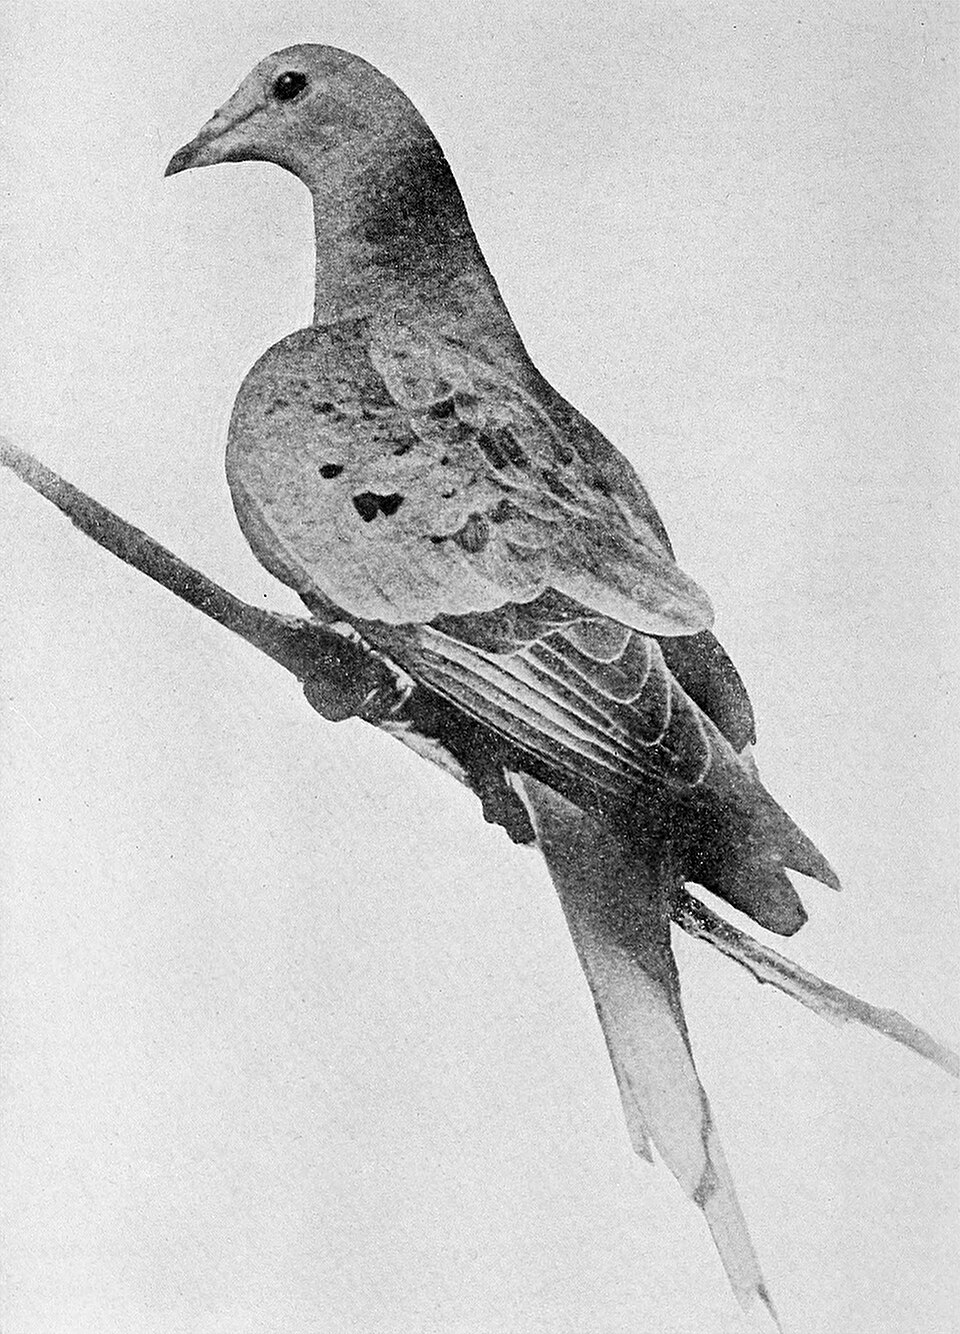
\includegraphics[width=0.4\linewidth]{images/book5/martha.jpg}\hspace{0.04\linewidth}
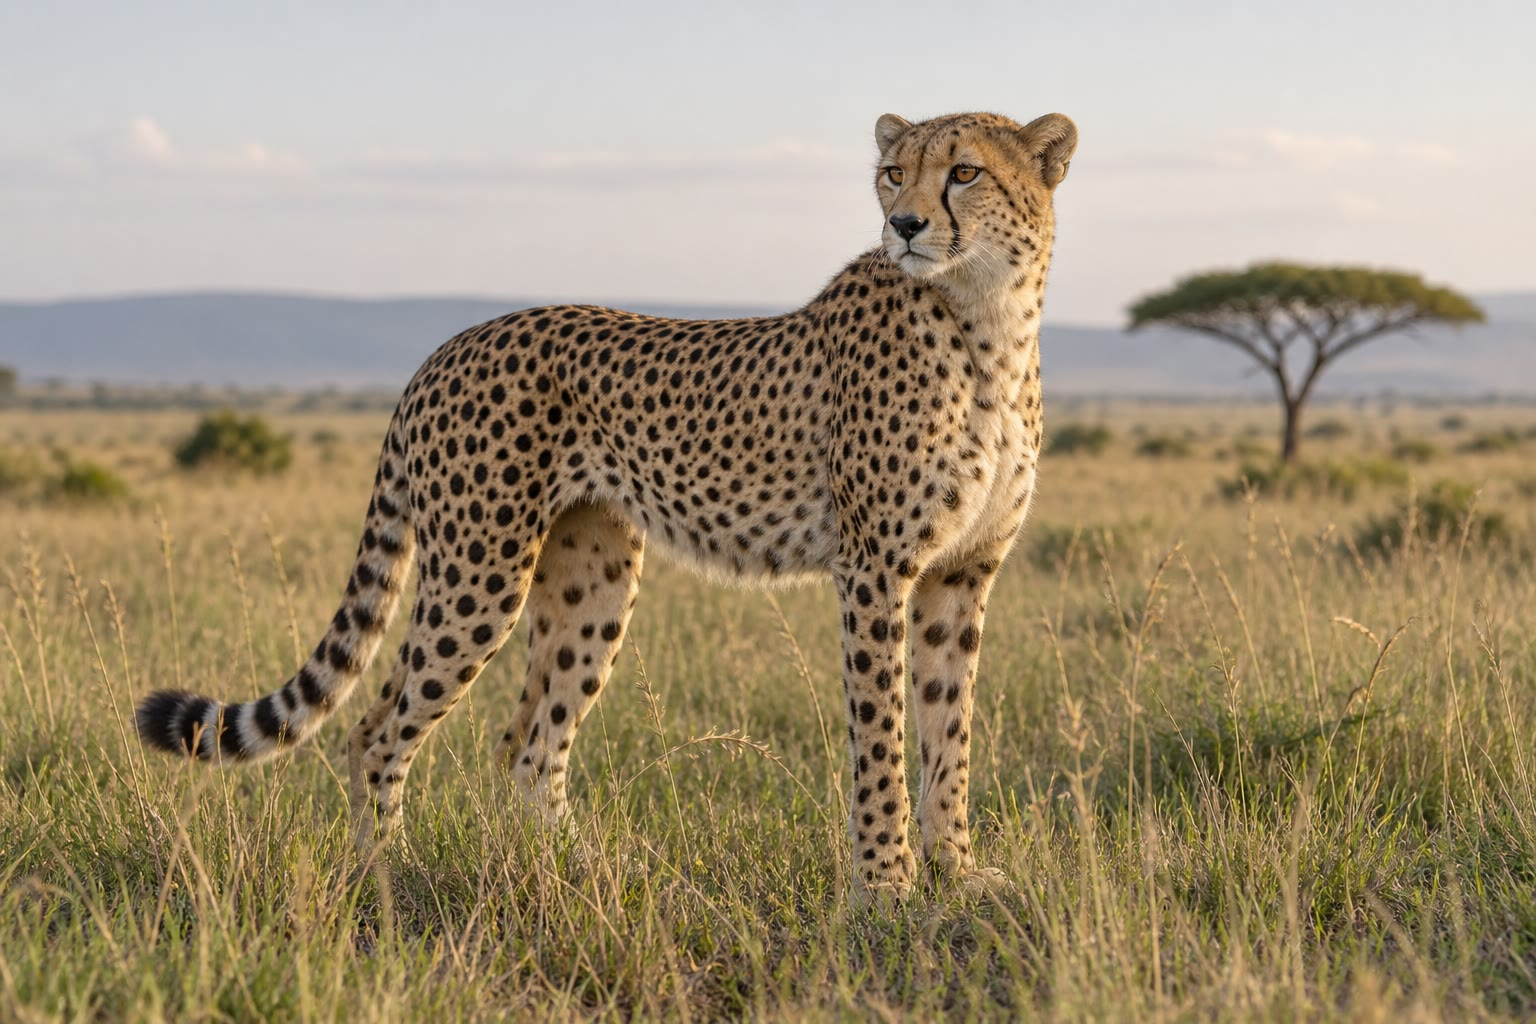
\includegraphics[width=0.52\linewidth]{images/book5/ai/b5-27-cheetah.jpg}

{\small Kiri: Martha, merpati penumpang terakhir, difoto di Kebun
Binatang Cincinnati pada 1912; spesiesnya pernah berjumlah miliaran dalam
ingatan orang yang masih hidup (foto oleh Enno Meyer, domain publik).
Kanan: seekor citah --- spesies yang melewati sebuah leher botol sekitar
sepuluh ribu tahun lalu dan individunya begitu serupa sehingga cangkok
kulit antara hewan yang tidak berkerabat pun tidak ditolak.}
\end{omfigure}

\section{Habitat: berapa luas, dan dalam bentuk apa}

\begin{proposition}[Spesies dan luas]\label{prop:b3:conservation-biology:area}
\index{hubungan spesies--luas}\index{pemecahan habitat}\index{biogeografi pulau}%
\index{koridor}\index{perdebatan SLOSS}\index{efek tepi}
Di seluruh pulau, dan di seluruh serpihan habitat yang berlaku seperti
pulau, jumlah spesies $S$ naik bersama luas $A$ sebagai sebuah hukum pangkat,
\[
S = c\,A^{z}, \qquad z \approx 0.15\text{--}0.35,
\]
yaitu \emph{\omterm{prop:b3:conservation-biology:area}{hubungan spesies--luas}} (Arrhenius, 1921; \omterm{prop:b3:conservation-biology:area}{biogeografi pulau}
MacArthur dan Wilson, 1967, menerangkannya sebagai perimbangan antara
imigrasi dan kepunahan, dengan kepunahan yang lebih cepat di pulau kecil).
Dengan $z = 0.25$, kehilangan \qty{90}{\%} luas sebuah habitat akhirnya
menghilangkan $1 - 0.1^{0.25} = \qty{44}{\%}$ spesiesnya; kehilangan
separuhnya menghilangkan \qty{16}{\%}. Kehilangannya tidak seketika ---
\emph{utang kepunahan} dibayar sepanjang berpuluh tahun ketika populasi
yang terlalu kecil bagi serpihannya menyusut --- dan \emph{pemecahan}
sebuah luas yang tetap menjadi kepingan menambahkan kehilangan tersendiri:
tiap serpihan menampung populasi yang lebih kecil, \emph{\omterm{prop:b3:conservation-biology:area}{efek tepi}}
(angin, panas, pemangsa, gulma) menembus ratusan meter ke dalam hutannya,
dan spesies yang memerlukan bagian dalamnya kehilangan lebih banyak
daripada yang diperhitungkan luasnya. Apakah satu suaka besar atau
beberapa suaka kecil dengan luas total yang sama menyelamatkan lebih
banyak spesies (perdebatan \emph{SLOSS}) bergantung pada spesiesnya: yang
besar menampung populasi yang lebih besar dan habitat bagian dalam, yang
kecil menyebarkan risiko malapetaka lalu mencuplik lebih banyak jenis
habitat. \emph{Koridor} yang menghubungkan serpihannya membiarkan individu
dan gen berpindah di antaranya, mengubah populasi yang terpencil menjadi
sebuah metapopulasi yang bagiannya dapat dihuni kembali setelah kepunahan
setempat dan diselamatkan dari silang dalam --- itulah sebabnya lahan di
antara suakanya menjadi sama pentingnya dengan suakanya sendiri.
\end{proposition}
\begin{proof}
Hukum pangkatnya bersifat empiris, dicocokkan pada sumbu log--log
terhadap kepulauan, danau, puncak gunung dan serpihan hutan di seluruh
dunia; nilai $z$ lebih rendah bagi kepingan sebuah daratan utama (imigrasi
menjaga spesiesnya tetap ada) dan lebih tinggi bagi pulau sejati.
Kehilangan pecahannya menyusul langsung: $S'/S = (A'/A)^{z}$. Mekanisme
\omterm{prop:b3:conservation-biology:area}{biogeografi pulau} diuji oleh Simberloff dan Wilson (1969), yang mengasapi
pulau bakau kecil di Florida, membunuh tiap artropoda, lalu menyaksikan
jumlah spesiesnya kembali ke nilai sebelumnya dalam setahun --- sebuah
kesetimbangan, dengan spesies yang berbeda daripada dahulu: jumlahnya
ditetapkan oleh luas dan jaraknya, jati dirinya oleh kebetulan.
\end{proof}

\begin{omfigure}
\begin{tikzpicture}
\begin{loglogaxis}[
  width=0.6\linewidth, height=5.4cm,
  axis x line=bottom, axis y line=left,
  xmin=0.5, xmax=20000, ymin=5, ymax=300,
  xlabel={luas (km$^2$)}, ylabel={jumlah spesies},
  xlabel style={font=\small, at={(axis description cs:0.5,-0.12)}, anchor=north}, ylabel style={font=\small},
  tick label style={font=\small}, xtick={1,10,100,1000,10000}, xticklabels={1,10,100,1000,10000}, ytick={10,30,100,300}, yticklabels={10,30,100,300},
  clip=false,
]
\addplot[very thick, omDef, domain=0.5:20000, samples=40] {20*x^0.25};
\addplot[only marks, mark=*, mark size=1.8pt, omDef!70!black] coordinates {(1,22) (3,24) (10,38) (30,44) (100,66) (300,80) (1000,110) (3000,150) (10000,190)};
\draw[dashed, gray] (axis cs:10000,5) -- (axis cs:10000,200) -- (axis cs:0.5,200);
\draw[dashed, gray] (axis cs:1000,5) -- (axis cs:1000,112.5) -- (axis cs:0.5,112.5);
\node[font=\scriptsize, omDef, anchor=south west] at (axis cs:1.2,215) {$S = c\,A^{0.25}$: kemiringan $z$ pada sumbu log};
\node[font=\scriptsize, anchor=west, align=left] at (axis cs:1200,40) {kehilangan \qty{90}{\%} luasnya:\\menahan $0.1^{0.25} = \qty{56}{\%}$\\spesiesnya};
\end{loglogaxis}
\end{tikzpicture}

{\small Hukum spesies--luas pada sumbu logaritmik. Kemiringannya adalah
eksponen $z$; darinya kehilangan spesies yang akhirnya diderita sebuah
habitat yang menyusut dapat dibaca --- sepersepuluh hutannya menahan
kira-kira separuh spesiesnya, dan bukan sepersepuluh seperti tebakan linier.}
\end{omfigure}

\begin{omfigure}
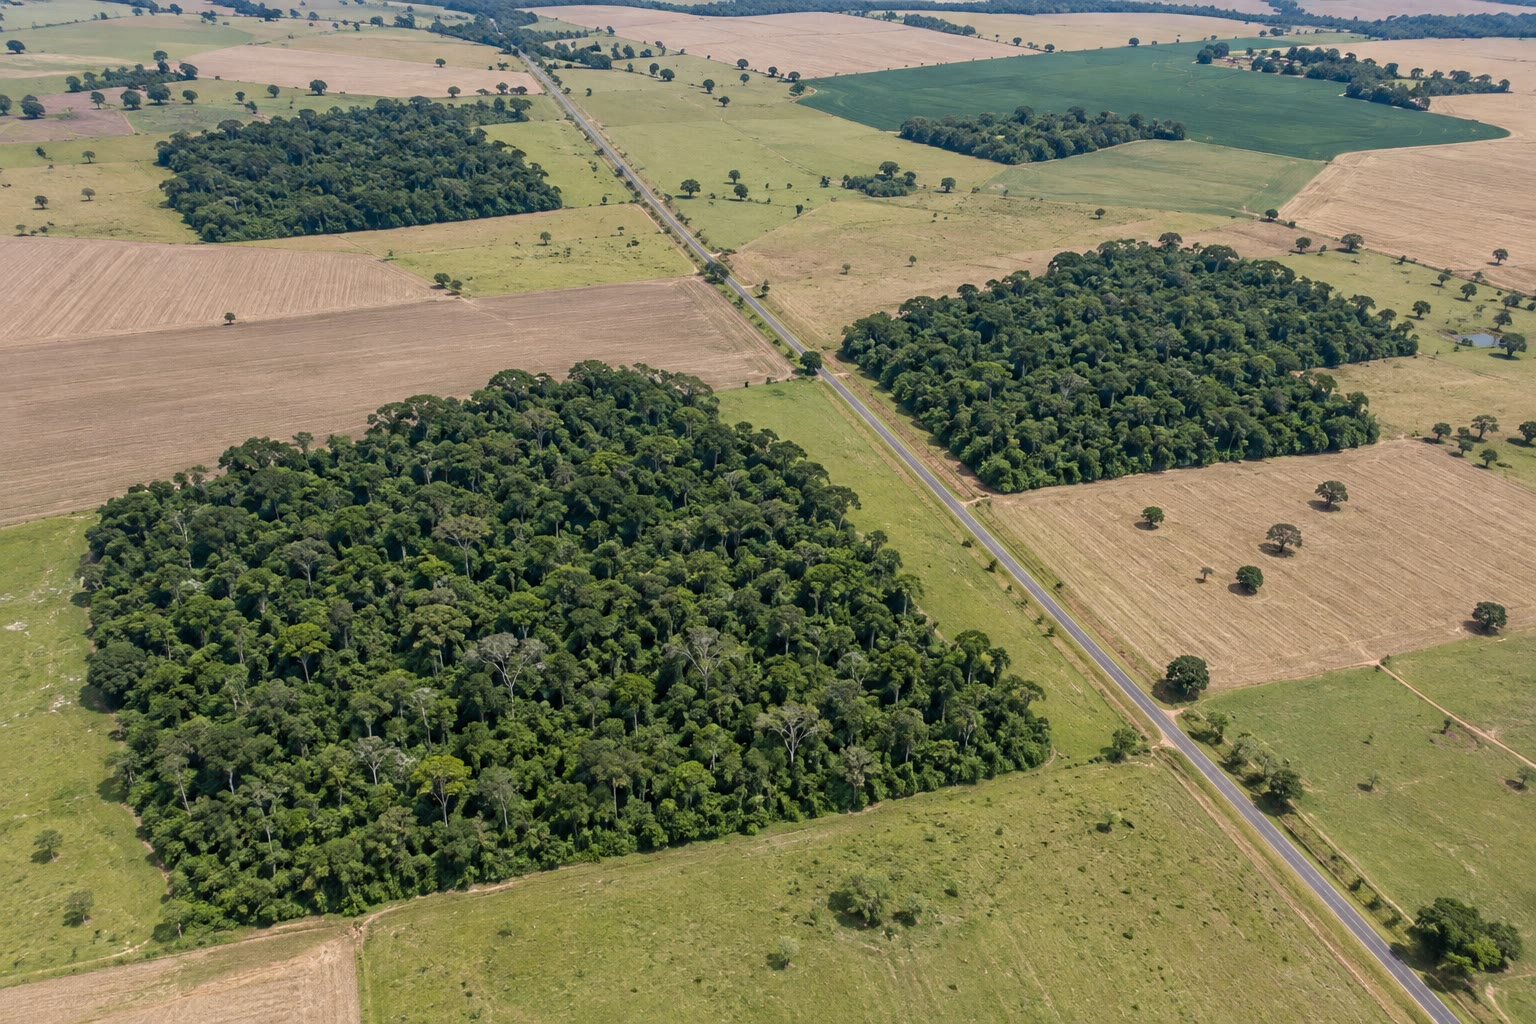
\includegraphics[width=0.6\linewidth]{images/book5/ai/b5-27-forest-fragments.jpg}

{\small Serpihan hutan di tengah lahan pertanian, dilihat dari udara: tiap
pulaunya menampung populasi yang lebih kecil daripada hutan utuhnya
dahulu, ditepii sebuah zona yang tidak dapat dipakai spesies bagian
dalamnya, dan dipisahkan oleh ladang yang tidak dapat diseberangi spesies
hutannya.}
\end{omfigure}

\section{Meramalkan dan mencegah}

\begin{method}[Analisis kelayakan populasi]\label{met:b3:conservation-biology:pva}
\index{analisis kelayakan populasi}\index{kepunahan semu}
Untuk menaksir risiko kepunahan sebuah populasi dan apa yang akan
menguranginya: (1) bangunlah model dinamikanya --- sebuah matriks
keselamatan dan kesuburan menurut umur atau tahapnya, seperti demografi
pada jilid Tahun~2, yang ditaksir dari individu bertanda sepanjang
beberapa tahun; (2) tambahkan stokastisitasnya --- yang demografis, dengan
mengundi nasib tiap individu secara acak, dan yang lingkungan, dengan
mengundi laju tiap tahun dari ragam yang teramati, disertai malapetaka
sesekali; (3) tambahkan kebergantungan kerapatan dan kemerosotan genetik
akibat silang dalam bila datanya memungkinkan; (4) simulasikan ribuan
lintasan dari ukuran sekarang sepanjang cakrawala yang diminati lalu
catatlah pecahan yang jatuh di bawah sebuah ambang \emph{\omterm{met:b3:conservation-biology:pva}{kepunahan semu}}
(yaitu ukuran yang darinya pemulihan dinilai mustahil); (5) ragamkan
masukannya --- keselamatan dewasa, keselamatan muda, luas habitat, sebuah
pemindahan sepuluh ekor hewan --- lalu lihatlah perubahan mana yang paling
mengurangi risikonya; di situlah upaya harus ditaruh. Keluarannya adalah
sebuah peluang dengan ketakpastian yang lebar, bukan sebuah ramalan;
nilainya bersifat pembanding, dan ia berulang kali menunjukkan bahwa
keselamatan dewasa, bukan kesuburan, adalah tuasnya pada spesies yang
berumur panjang, dan itulah sebabnya tali pancing membunuh populasi
albatros yang bertelur satu butir tiap dua tahun lebih cepat daripada
kehilangan sarang mana pun.
\end{method}

\begin{proposition}[Waktu sampai punah]\label{prop:b3:conservation-biology:time}
\index{waktu kepunahan}
Bagi sebuah populasi yang berayun karena lingkungannya berayun, dengan
laju pertumbuhan rata-rata $\bar r$ dekat nol dan ragam $\sigma^{2}$ pada
laju pertumbuhan tahunannya, logaritma ukuran populasinya menempuh sebuah
pengembaraan acak dengan hanyutan, dan waktu harapan sampai punah dari
ukuran $N$ tumbuh hanya sebagai \emph{logaritma} $N$ bila $\bar r < 0$ ---
melipatduakan populasinya menambahkan jumlah tahun yang tetap --- dan
sebagai sebuah \emph{pangkat} $N$ bila $\bar r > 0$, dengan eksponen
$2\bar r/\sigma^{2} - 1$; di bawah \omterm{def:b3:conservation-biology:small}{stokastisitas demografi} saja ia tumbuh
\emph{secara eksponensial} bersama $N$, sehingga sebuah populasi yang aman
dari kebetulan demografis pada seratus ekor masih dapat hilang karena ragam
lingkungan pada sepuluh ribu ekor. Akibat praktisnya adalah bahwa
menurunkan ragam pertumbuhan sebuah populasi --- meredamnya terhadap tahun
yang buruk dengan habitat yang lebih luas, tapak yang lebih banyak,
makanan yang lebih beragam --- dapat berbuat lebih banyak bagi
kelestariannya daripada menaikkan rata-ratanya.
\end{proposition}
\admitted

\begin{omfigure}
\begin{tikzpicture}
\begin{semilogyaxis}[
  width=0.62\linewidth, height=5.4cm,
  axis x line=bottom, axis y line=left,
  xmin=0, xmax=50, ymin=1, ymax=3000,
  xlabel={tahun}, ylabel={ukuran populasi},
  xlabel style={font=\small, at={(axis description cs:0.5,-0.12)}, anchor=north}, ylabel style={font=\small},
  tick label style={font=\small}, xtick={0,10,20,30,40,50}, ytick={1,10,100,1000}, yticklabels={1,10,100,1000},
  clip=false,
]
\addplot[thick, omDef] coordinates {(0,200) (2,240) (4,190) (6,260) (8,300) (10,220) (12,180) (14,250) (16,330) (18,280) (20,350) (22,300) (24,260) (26,340) (28,420) (30,380) (32,450) (34,400) (36,520) (38,480) (40,560) (42,500) (44,600) (46,650) (48,610) (50,700)};
\addplot[thick, omThm] coordinates {(0,200) (2,150) (4,180) (6,120) (8,90) (10,110) (12,70) (14,50) (16,60) (18,35) (20,40) (22,25) (24,18) (26,22) (28,12) (30,8) (32,9) (34,5) (36,3) (38,2) (40,1)};
\addplot[thick, omMeth!70!black] coordinates {(0,200) (2,210) (4,170) (6,200) (8,140) (10,160) (12,120) (14,140) (16,90) (18,110) (20,80) (22,95) (24,60) (26,75) (28,50) (30,55) (32,40) (34,45) (36,30) (38,35) (40,28) (42,30) (44,22) (46,25) (48,20) (50,22)};
\draw[dashed, gray] (axis cs:0,20) -- (axis cs:50,20); \node[font=\scriptsize, gray, anchor=north east] at (axis cs:49,18) {ambang kepunahan semu};
\node[font=\scriptsize, omDef, anchor=west] at (axis cs:50.5,700) {$\bar r > 0$: lestari};
\node[font=\scriptsize, omMeth!70!black, anchor=west] at (axis cs:50.5,22) {$\bar r \approx 0$: menghanyut turun};
\node[font=\scriptsize, omThm, anchor=west] at (axis cs:40.5,1.3) {$\bar r < 0$: lenyap dalam 40 tahun};
\end{semilogyaxis}
\end{tikzpicture}

{\small Tiga lintasan simulasi dari dua ratus ekor hewan yang sama, yang
berbeda hanya pada laju pertumbuhan rata-ratanya; sebuah analisis
kelayakan menjalankan ribuan lintasan seperti ini lalu menghitung berapa
yang melintasi ambangnya. Ragam dari tahun ke tahun itulah yang membuat
kasus tengahnya pun menjadi sebuah judi.}
\end{omfigure}

\begin{definition}[Perkakas konservasi]\label{def:b3:conservation-biology:tools}
\index{Daftar Merah IUCN}\index{spesies invasif}%
\index{konservasi ex situ}\index{pembiakan dalam kurungan}%
\index{reintroduksi}\index{pengliaran kembali}\index{riam trofik}
\emph{Daftar Merah IUCN} menggolongkan spesies menurut kriteria
kuantitatif: kemerosotan sebesar \qty{30}{\%}, \qty{50}{\%} atau
\qty{80}{\%} sepanjang sepuluh tahun atau tiga generasi, sebaran di bawah
\qty{20000}{}, \qty{5000}{} atau \qty{100}{km^2}, populasi di bawah
\qty{10000}{}, \qty{2500}{} atau \qty{250}{} individu dewasa, atau sebuah
peluang kepunahan yang dimodelkan, menempatkan sebuah spesies sebagai
Rentan, Terancam atau Terancam Kritis; seperempat mamalia dan seperdelapan
burung memenuhinya. Penyebabnya adalah hilangnya habitat lebih dahulu,
lalu panen berlebih, \emph{spesies invasif} (pemangsa dan pesaing yang
dibawa ke pulau yang spesiesnya tidak pernah menjumpainya: tikus, kucing
dan cerpelai telah mengambil sebagian besar burung Selandia Baru, seekor
ular pohon cokelat sebagian besar burung Guam), pencemaran dan perubahan
iklim. Tanggapannya: kawasan lindung yang meliputi seperenam daratan;
pengendalian atau pemberantasan penyerbunya (seratus lima puluh pulau
dibersihkan dari tikus); konservasi \emph{ex situ} --- bank benih yang
menyimpan sejuta aksesi di dalam sebuah lumbung di beku abadi Arktik,
embrio beku, dan \emph{pembiakan dalam kurungan} dengan silsilah yang
dikelola untuk memperkecil kekerabatan, yang membawa kembali kondor
California dari dua puluh dua ekor pada 1987 dan feret berkaki hitam dari
delapan belas ekor; \emph{reintroduksi}, yang berhasil kira-kira sepertiga
kalinya dan lebih sering bila penyebab kehilangan aslinya telah
disingkirkan; dan \emph{pengliaran kembali}, yaitu kembalinya hewan besar
dan proses yang mereka gerakkan --- serigala Yellowstone, yang
pemangsaannya serta rasa takut akan pemangsaan itu memindahkan rusa
wapitinya dari tepi sungai lalu membiarkan dedalu, aspen, berang-berang
dan burung penyanyi kembali, yaitu sebuah \emph{riam trofik} yang berjalan
dari seekor karnivora sampai ke bentuk sebuah sungai.
\end{definition}

\begin{omfigure}
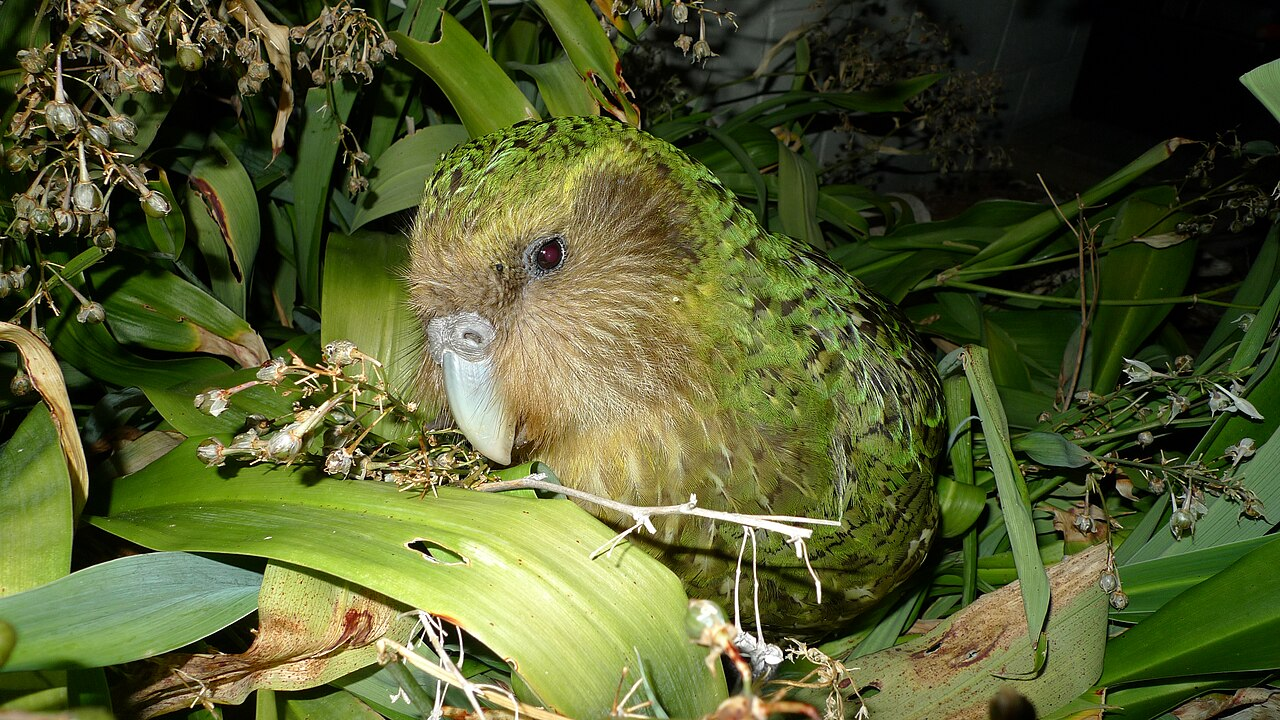
\includegraphics[width=0.46\linewidth]{images/book5/kakapo-sirocco.jpg}\hspace{0.04\linewidth}
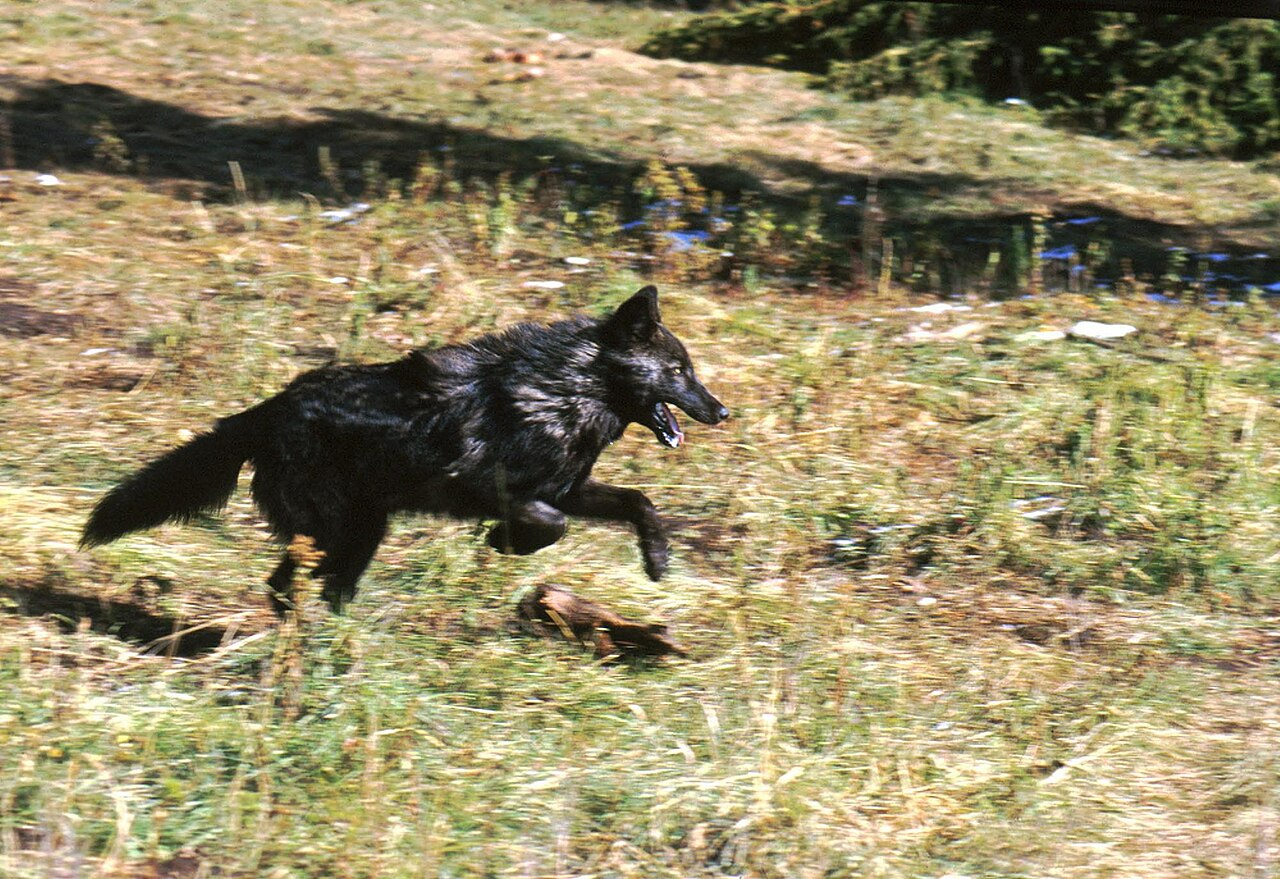
\includegraphics[width=0.46\linewidth]{images/book5/yellowstone-wolves-1996.jpg}

{\small Kiri: Sirocco, seekor kakapo --- satu dari lima puluh satu yang
selamat pada 1995, kini satu dari sekitar dua ratus lima puluh, yang tiap
ekornya dinamai dan dipantau di pulau bebas pemangsa (foto: Departemen
Konservasi Selandia Baru, CC BY 2.0). Kanan: serigala di Yellowstone
pada 1996, musim dingin pertama setelah \omterm{def:b3:conservation-biology:tools}{reintroduksinya} (foto: National
Park Service, domain publik).}
\end{omfigure}

\begin{example}[Tiga pemulihan]\label{ex:b3:conservation-biology:recoveries}
Kakapo: lima puluh satu ekor pada 1995, semuanya dipindahkan ke pulau yang
telah dibersihkan dari pemangsa; tiap ekor membawa pemancar, tiap sarang
diawasi kamera, anaknya dibesarkan dengan tangan bila induknya gagal,
jantannya diberi makan agar mencapai kondisi berbiak pada tahun ketika
pohon rimu berbuah, dan silsilahnya dikelola agar gen langka jantan
Fiordland terakhir tetap berada di dalam populasinya; genom tiap kakapo
telah diurutkan. Kini dua ratus lima puluh ekor, dan sebuah $N_{e}$ yang
menurut genomnya mendekati seratus. Jenjang Amerika: lima belas ekor pada
1941, satu kawanan bermigrasi tunggal, dibiakkan di dalam kurungan dari
telur yang diambil dari sarang liar, diajari rute migrasi baru di belakang
pesawat ultraringan, dan kini sekitar delapan ratus ekor. Paus bungkuk:
diburu sampai tinggal beberapa ribu ekor, dilindungi pada 1966, dan kini
melampaui seratus ribu, yaitu sebuah kenaikan mendekati \qty{8}{\%}
setahun yang menunjukkan apa yang dilakukan seekor hewan berumur panjang
ketika satu-satunya penyebab kemerosotannya disingkirkan. Tiap pemulihan
berongkos puluhan juta dan berpuluh tahun; aritmetika bab ini mengatakan
mengapa upayanya harus dikeluarkan sebelum jumlahnya mencapai pusarannya,
dan mengapa itu lebih murah daripada penyelamatan mana pun di kemudian hari.
\end{example}

\begin{omfigure}
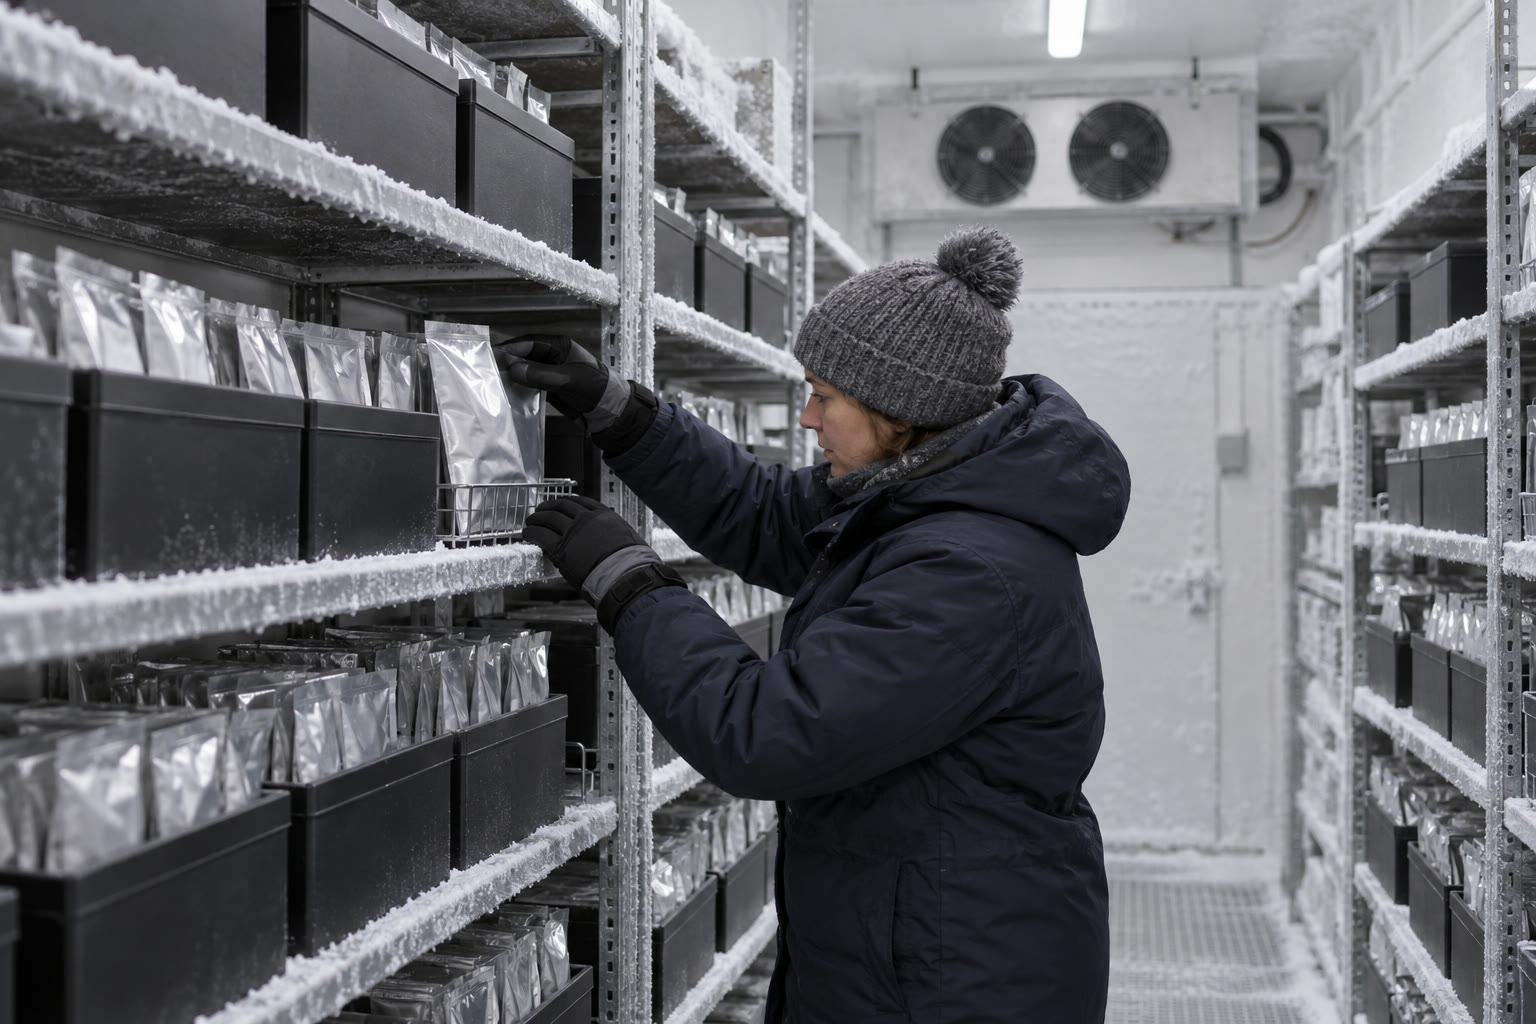
\includegraphics[width=0.56\linewidth]{images/book5/ai/b5-27-seed-vault.jpg}

{\small Sebuah lumbung benih di dalam beku abadi: duplikat sejuta aksesi
tanaman pangan dan tumbuhan liar, disimpan pada \qty{-18}{\celsius}
terhadap hilangnya koleksi asalnya --- konservasi sebagai asuransi, pada
skala genom sebuah spesies.}
\end{omfigure}

\begin{remark}[Aritmetika penjagaan]\label{rem:b3:conservation-biology:remark}
Tiap bab rangkaian ini berakhir pada sebuah angka, dan bab ini berakhir
pada beberapa angka: sebuah ukuran efektif, sebuah \omterm{thm:b3:conservation-biology:ne}{koefisien silang dalam}
yang naik sebesar $1/2N_{e}$ tiap generasi, sebuah eksponen $z$ yang
mengubah hektare yang hilang menjadi spesies yang hilang, sebuah peluang
kepunahan sepanjang satu abad. Semuanya kasar --- cacah jiwanya tidak
pasti, ragamnya ditebak, modelnya sebuah karikatur --- dan semuanya itulah
yang mengubah sebuah perasaan tentang burung yang lenyap menjadi sebuah
keputusan tentang lima puluh hektare mana yang harus dibeli dan delapan
ekor hewan mana yang harus dipindahkan. Biologinya adalah biologi yang
sama dengan sisa buku ini: hanyutan, seleksi, demografi, perilaku,
kebergantungan sebuah populasi pada habitatnya dan sebuah habitat pada
populasinya. Yang baru hanyalah kemendesakannya, dan kenyataan bahwa
percobaannya sedang dijalankan sekali saja, tanpa kendali, pada spesies
yang tersisa.
\end{remark}

\section{Latihan}

\begin{exercise}[$\star$]\label{exo:b3:conservation-biology:1}
Definisikanlah \omterm{def:b3:conservation-biology:small}{stokastisitas demografi}, \omterm{def:b3:conservation-biology:small}{stokastisitas lingkungan} dan \omterm{def:b3:conservation-biology:small}{efek
Allee}, lalu berilah satu contoh masing-masing dari bab ini.
\end{exercise}

\begin{exercise}[$\star$]\label{exo:b3:conservation-biology:2}
Apakah \omterm{thm:b3:conservation-biology:ne}{ukuran populasi efektif} itu, dan sebutkanlah tiga ciri sebuah
populasi nyata yang membuatnya lebih kecil daripada cacah jiwanya.
\end{exercise}

\begin{exercise}[$\star$]\label{exo:b3:conservation-biology:3}
Nyatakanlah hukum spesies--luas. Bila $z = 0.25$, berapa bagian spesies
yang ditahan sebuah habitat setelah kehilangan separuh luasnya? Sembilan
persepuluh luasnya? Sembilan puluh sembilan perseratus luasnya?
\end{exercise}

\begin{exercise}[$\star$]\label{exo:b3:conservation-biology:4}
Jelaskanlah kaidah 50/500, dan apa yang dilindungi tiap angkanya.
\end{exercise}

\begin{exercise}[$\star\star$]\label{exo:b3:conservation-biology:5}
Sekawanan 200 anjing laut gajah memiliki 8 jantan pembiak dan 120 betina
pembiak. Hitunglah $N_{e}$ dan kehilangan keheterozigotan tiap
generasinya. Berapa generasi untuk kehilangan seperempatnya?
\end{exercise}

\begin{exercise}[$\star\star$]\label{exo:b3:conservation-biology:6}
Sebuah populasi berjumlah 1000, 1000, 20, 1000, 1000 pada lima generasi
berturut-turut. Hitunglah $N_{e}$ sepanjang rentang itu, dan
keheterozigotan yang ditahan, lalu bandingkanlah dengan 1000 yang tetap.
\end{exercise}

\begin{exercise}[$\star\star$]\label{exo:b3:conservation-biology:7}
Dua puluh lima ekor puma Florida dengan $N_{e} \approx 10$: berapa silang
dalam yang tertimbun dalam 5 generasi? Bila kebugaran turun \qty{5}{\%}
tiap \qty{10}{\%} nilai $F$, sudah berapa banyak kebugaran yang turun? Apa
yang dilakukan penambahan delapan betina tak berkerabat terhadap $F$ pada
generasi berikutnya?
\end{exercise}

\begin{exercise}[$\star\star$]\label{exo:b3:conservation-biology:8}
Yellowstone: 31 serigala dilepaskan pada 1995--96, sekitar 100 ekor di
dalam tamannya pada 2003. Taksirlah $r$; berapa banyak yang akan ada pada
2020 bila pertumbuhannya berlanjut, dan mengapa ia tidak berlanjut?
\end{exercise}

\begin{exercise}[$\star\star$]\label{exo:b3:conservation-biology:9}
Golongkanlah menurut kriteria IUCN di dalam bab ini: (a) seekor katak yang
populasinya jatuh \qty{60}{\%} dalam sepuluh tahun; (b) sebuah tumbuhan
dengan 180 individu dewasa; (c) seekor ikan yang sebarannya
\qty{3000}{km^2}; (d) seekor burung dengan \num{30000} individu yang
merosot \qty{10}{\%} tiap dasawarsa.
\end{exercise}

\begin{exercise}[$\star\star\star$]\label{exo:b3:conservation-biology:10}
Sebuah populasi berisi $N$ pasangan yang masing-masing menghasilkan,
dengan peluang $1/2$, dua anak yang selamat dan selebihnya tidak satu pun
(\omterm{def:b3:conservation-biology:small}{stokastisitas demografi}). Hitunglah peluang bahwa seluruh populasinya
gagal dalam satu generasi bagi $N = 2$, $5$, $10$, $20$, lalu berilah
komentar tentang bagaimana risiko demografis berskala bersama $N$.
\end{exercise}

\begin{exercise}[$\star\star\star$]\label{exo:b3:conservation-biology:11}
Hukum spesies--luas dengan $z = 0.25$, dan sebuah hutan yang dipotong
menjadi 10 serpihan terpencil yang sama luasnya. Bandingkanlah spesies
yang diharapkan pada satu serpihan dengan sepersepuluh spesies asalnya,
lalu berilah alasan mengapa total di seluruh serpihannya bukan sekadar
jumlah asalnya --- apa yang menentukan apakah serpihannya bersama-sama
menampung lebih banyak atau lebih sedikit spesies daripada hutan utuhnya dahulu?
\end{exercise}

\begin{exercise}[$\star\star\star$]\label{exo:b3:conservation-biology:12}
Mengapa menambahkan beberapa migran tiap generasi ($m N_{e} \approx 1$)
sebagian besar menghentikan hilangnya keragaman pada sebuah populasi
kecil, dan apa ongkosnya bagi penyesuaian setempat? Pakailah perimbangan
antara hanyutan, $1/2N_{e}$, dan pecahan alel yang diganti para migran,
$m$, untuk beralasan.
\end{exercise}

\section{Soal: Lima Puluh dan Lima Ratus}

\begin{problem}[{Soal akhir pekan --- sebuah program pemulihan dalam
angka: ukuran efektif sebuah populasi burung nuri yang diselamatkan dan
silang dalamnya, sebuah penyelamatan genetik, spesies yang akan ditahan
sebuah hutan yang menyusut, pertumbuhan serigala yang direintroduksi,
serta kategori dan ongkosnya, yang berakhir pada $N_{e}$, silang dalam
setelah sepuluh generasi dan pecahan spesies yang ditahan}]
\label{pb:b3:conservation-biology:1}
Data: sebuah populasi burung nuri berisi 60 ekor dewasa, 20 jantan dan 40
betina, semuanya berbiak; waktu generasinya \qty{10}{yr}. Riwayat
populasinya sepanjang lima generasi terakhir: 500, 100, 60, 51, 60.
Depresi silang dalam: kebugaran turun \qty{6}{\%} tiap \qty{0.1}{} nilai
$F$. Penyelamatan: 10 ekor burung tak berkerabat ditambahkan pada 60 ekor.
Hutan: \qty{2000}{km^2} disusutkan menjadi \qty{300}{km^2}, $z = 0.25$;
spesiesnya kini 180. Serigala: 31 ekor dilepaskan, 100 ekor setelah 8
tahun, daya dukung di dalam tamannya sekitar 120 ekor. Ongkos: empat juta
dolar setahun bagi burung nurinya.

\medskip
\noindent\textbf{Bagian I --- Ukuran efektif.}
\begin{enumerate}
  \item $N_{e}$ dari \omterm{thm:b3:conservation-biology:ne}{nisbah kelamin} 60 ekor yang sekarang. Bandingkanlah
        dengan cacah jiwanya.
  \item $N_{e}$ \omterm{thm:b3:conservation-biology:ne}{rata-rata harmonik} sepanjang lima generasi riwayatnya.
        Generasi mana yang menguasainya?
  \item Silang dalam yang tertimbun sepanjang lima generasi itu, memakai
        $N_{e}$ \omterm{thm:b3:conservation-biology:ne}{rata-rata harmoniknya} (rumus eksak dan hampiran liniernya).
  \item Kebugaran yang hilang karena silang dalam itu.
  \item Keheterozigotan yang ditahan setelah lima generasi itu, sebagai
        sebuah pecahan dari nilai asalnya.
  \item Bila populasinya kini ditahan pada 60 ekor dengan \omterm{thm:b3:conservation-biology:ne}{nisbah kelamin}
        yang sekarang, nilai $F$ berapa yang akan dicapainya dalam sepuluh
        generasi lagi, dan berapa kebugaran yang hilang? Berapa tahunkah itu?
\end{enumerate}

\medskip
\noindent\textbf{Bagian II --- Penyelamatan.}
\begin{enumerate}[resume]
  \item Sepuluh ekor burung tak berkerabat bergabung dengan 60 ekor.
        Pecahan alel pada generasi berikutnya yang berasal dari
        pendatangnya kira-kira $10/70$; \omterm{thm:b3:conservation-biology:ne}{koefisien silang dalam} anak dengan
        satu induk asli dan satu induk pendatang adalah $0$. Taksirlah
        rata-rata $F$ populasinya pada generasi berikutnya bila
        perkawinannya acak.
  \item Jelaskanlah mengapa $F$ jatuh seketika tetapi keheterozigotannya
        naik hanya seiring menyebarnya alel para migran, dan mengapa
        penyelamatan kedua mungkin diperlukan.
  \item Untuk mencapai $N_{e} = 500$ dengan \omterm{thm:b3:conservation-biology:ne}{nisbah kelamin} seimbang,
        berapa ekor dewasa yang diperlukan? Pada $r = \qty{0.05}{yr^{-1}}$
        dari 70 ekor burung, berapa tahun?
  \item Programnya mengambil telur dari induk yang buruk untuk dibesarkan
        dengan tangan, yang menaikkan rata-rata cacah anak yang
        meninggalkan sarang tiap pasangan tetapi menyeragamkan ukuran
        keluarganya. Mengapa penyeragaman ukuran keluarga \emph{menaikkan}
        $N_{e}$ di atas cacah jiwanya (menuju $2N$)?
  \item Jantan terakhir sebuah galur selatan yang khas mandul di alam
        liar. Usulkanlah dua campur tangan dan ongkosnya bagi lungkang gennya.
  \item Pada empat juta dolar setahun sepanjang 40 tahun sampai mencapai
        $N_{e} = 500$, berapa ongkos totalnya, dan ongkos tiap burung yang
        ditambahkan? Mahalkah itu? Terhadap apa?
\end{enumerate}

\medskip
\noindent\textbf{Bagian III --- Hutan.}
\begin{enumerate}[resume]
  \item Pecahan spesies yang akan ditahan hutannya pada \qty{300}{km^2};
        jumlah spesies yang diharapkan, dan utang kepunahannya (spesies
        yang ada sekarang yang akan hilang).
  \item Bila sebagai gantinya \qty{300}{km^2} itu berupa tiga serpihan
        terpencil seluas \qty{100}{km^2}, berapa spesies tiap serpihannya;
        berapa totalnya bila serpihannya menampung spesies yang seluruhnya
        berbeda; berapa totalnya bila serupa. Apa yang menentukannya?
  \item Sebuah koridor seluas \qty{20}{km^2} menyambung ketiga
        serpihannya. Perlakukanlah semuanya sebagai satu luas
        \qty{320}{km^2}: berapa spesies yang diharapkan. Bandingkanlah
        dengan kasus spesies serupa pada pertanyaan~14.
  \item Pemangsa terbesar hutannya memerlukan \qty{50}{km^2} tiap pasangan
        dan $N_{e}$ sebesar 50 agar lestari. Dapatkah seluruh
        \qty{300}{km^2} menampungnya? Dapatkah sebuah serpihan? Apa arti
        hal ini bagi luas berbanding jumlah spesies sebagai sebuah kriteria?
  \item Taksirlah berapa lama utang kepunahannya dibayar bila spesies yang
        hilang memiliki populasi yang merosot \qty{3}{\%} setahun dari 200
        ekor menuju sebuah ambang \omterm{met:b3:conservation-biology:pva}{kepunahan semu} sebesar 10 ekor.
  \item Mengapa hukum spesies--luas meremehkan kehilangannya ketika
        pemecahan menambahkan \omterm{prop:b3:conservation-biology:area}{efek tepi}, dan melebih-lebihkannya ketika
        lahan di sekelilingnya sebagian masih dapat dipakai?
\end{enumerate}

\medskip
\noindent\textbf{Bagian IV --- Serigala dan daftar.}
\begin{enumerate}[resume]
  \item Serigala: berapa $r$ dari $31 \to 100$ dalam 8 tahun, dan waktu
        lipat duanya.
  \item Pertumbuhan logistik menuju $K = 120$: berapa populasinya setelah
        8 tahun dengan pertumbuhan logistik alih-alih eksponensial, mulai
        dari 31 ekor dengan nilai $r$ pada pertanyaan~19 (pakailah
        $N(t) = K/[1 + (K/N_{0} -
        1)\mathrm{e}^{-rt}]$). Mana yang lebih cocok dengan 100 yang
        teramati, dan apa arti hal itu bagi kebergantungan kerapatan pada
        tahun-tahun pertamanya?
  \item Rusa wapitinya berjumlah \num{17000} ekor pada 1995 dan
        \num{4000} ekor pada 2015. Berapa laju kemerosotan tahunan
        rata-ratanya. Berapa banyak darinya yang dapat dijelaskan serigala
        yang memakan \num{20} ekor rusa wapiti tiap ekor setahun pada 100
        ekor serigala?
  \item Golongkanlah burung nurinya (60 individu dewasa) dan pemangsa
        hutannya sebelum penyelamatan menurut kriteria IUCN.
  \item Merpati penumpang: lima miliar ekor pada 1800, punah pada 1914.
        Bila kemerosotannya eksponensial sejak 1870, ketika masih ada
        miliaran ekor, sampai satu ekor pada 1914, laju tahunan berapa yang
        tersirat? Mengapa \omterm{def:b3:conservation-biology:small}{efek Allee} membuat dasawarsa terakhirnya lebih
        cepat daripada eksponensial?
  \item Jelaskanlah dalam satu paragraf mengapa sebuah PVA akan mengatakan
        merpati penumpang aman pada 1850, dan apa yang akan terlewatkan olehnya.
  \item Ringkaslah: nilai $N_{e}$ yang sekarang (pertanyaan~1), nilai $F$
        setelah sepuluh generasi lagi pada 60 ekor (pertanyaan~6), dan
        pecahan spesies yang ditahan hutan yang menyusut itu (pertanyaan~13).
\end{enumerate}
\end{problem}
